\section{671 --- Second Minimum Node In a Binary Tree}
Given a non-empty special binary tree consisting of nodes with the non-negative value, where each node in this tree has exactly \textbf{two} or \textbf{zero} sub-node. If the node has \textbf{two} sub-nodes, then this node's value is the smaller value among its two sub-nodes. 

More formally, the property \lstinline[language=Java, basicstyle=\small\ttfamily, keywordstyle=\bfseries\color{green!40!black}]|root.val = min(root.left.val, root.right.val)| always holds.

Given such a binary tree, you need to output the second minimum value in the set made of all the nodes' value in the whole tree.

If no such second minimum value exists, output $-1$ instead.

\paragraph{Example 1:}

\begin{flushleft}

\textbf{Input}:
\begin{figure}[H]
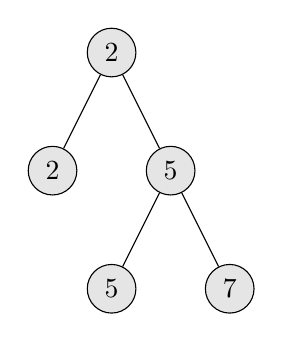
\begin{tikzpicture}
[every node/.style={draw, circle, fill=gray!20!, minimum size=5mm}]
\node{2}
child{node{2}}
child{node{5} child{node{5}} child{node{7}} };
\end{tikzpicture}
\end{figure} 

\textbf{Output}: 5

\textbf{Explanation}: The smallest value is 2, the second smallest value is 5.

\end{flushleft} 

\paragraph{Example 2:}

\begin{flushleft}

\textbf{Input}: 

\begin{figure}[H]
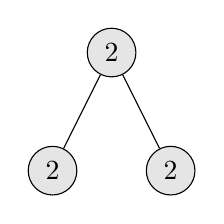
\begin{tikzpicture}
[every node/.style={draw, circle, fill=gray!20!, minimum size=5mm}]
\node{2}
child{node{2}}
child{node{2}};
\end{tikzpicture}
\end{figure}

\textbf{Output}: $-1$

\textbf{Explanation}: The smallest value is 2, but there isn't any second smallest value.
\end{flushleft}

\subsection{Depth First Search}
The problem asks for the 2nd minimum value, thus we may need to track both minimum, say, $x$, and 2nd minimum value, say $y$, at same time. From the property of the tree, we can easily know that the value of the root node is the minimum value of entire tree. Thus, $x$ will be the value of the root node.

When traversing the tree to a node, say $t$, if \lstinline[language=Java, basicstyle=\small\ttfamily, keywordstyle=\bfseries\color{green!40!black}]|t.val > x|, we know all values in the subtree root at $t$ are at least \lstinline[language=Java, basicstyle=\small\ttfamily, keywordstyle=\bfseries\color{green!40!black}]|t.val|, so there cannot be a better candidate for the second minimum in this subtree than \lstinline[language=Java, basicstyle=\small\ttfamily, keywordstyle=\bfseries\color{green!40!black}]|t.val|. Hence, we do not need to search this subtree.

Also, as we only care about the second minimum $y$, we do not need to record any values that are larger than our current candidate for the 2nd minimum value.

\setcounter{lstlisting}{0}
\begin{lstlisting}[style=customc, caption={DFS}]
int findSecondMinimumValue( TreeNode* root )
{
    int ans = -1;

    //root->val is the global minimum value
    //of entire tree
    dfs( root, root->val, ans );

    //since the tree only contains
    //non-negative number
    //if ans < 0, 2nd minimum has not been found
    return ans < 0 ? -1 : ans;
}

void dfs( TreeNode* node, int min_v, int& y )
{
    if( node )
    {
        if( node->val > min_v )
        {
            if( ( y < 0 ) || ( y > node->val ) )
            {
                //y < 0 means this is the
                //firt time to set y,
                //i.e. 2nd minimum value
                y = node->val;
            }
        }
        else if( node->val == min_v )
        {
            //recursively go to
            //left and right subtree
            dfs( node->left, min_v, y );
            dfs( node->right, min_v, y );
        }
    }
}
\end{lstlisting}